\section{Organizzazione del lavoro e sviluppo}
\label{organizzazionelavoro}

\subsection{Progettazione}
Nella fase iniziale si sono individuate capacità e punti di forza dei membri del gruppo.
In seguito a ciò si è deciso di non affidare a ciascuno una parte ben precisa del progetto ma di svolgerlo nella sua interezza in gruppo, in modo da mantenere la coerenza del codice e delle idee su tutto il piano lavorativo.
Questa decisione inoltre garantisce che ogni membro del gruppo abbia lavorato su tutte le parti principali del progetto.
Abbiamo deciso di svolgere il lavoro in parallelo con le lezioni del corso, usando quindi una strategia di progettazione classica:
\begin{enumerate}
\item Codifica pagine HTML;
\item Codifica pagine CSS;
\item Creazione e popolamento Database;
\item Codifica JavaScript;
\item Codifica pagine PHP.
\end{enumerate}
Punto fondamentale degno di nota è l’accessibilità. Essa non è posta nell’indice della progettazione appena descritto, poiché sono stati fatti test continui ad ogni passo della progettazione.
Così facendo, ogni blocco di lavoro compiuto risulta accessibile e valido.
Questo ci ha consentito di non dover tornare sui nostri passi in fasi più avanzate del progetto, ma poter contare su una base di lavoro effettuato in modo costante.

Nello specifico sono state progettate le pagine dedicate alla due funzionalità più importanti del sito: la prenotazione della visita e il consulto online.
I punti cardine di queste due pagine sono:
\begin{itemize}
\item \textbf{Confidenzialità:} le informazioni relative alle prenotazioni e tutte le conversazioni tra dottore e utente possono essere accedute solo dai diretti interessati. Questa caratteristica è garantita dal fatto che l’accesso alle due pagine di prenotazione e consulti è consentito solo agli utenti registrati;

%AGGIUNGERE IMMAGINE PRENOTAZIONI

\item \textbf{Semplicità:} la pagina di consulti online utilizza un singolo form sul quale poter scrivere il proprio messaggio. Una volta fatto ciò la conversazione viene mostrata secondo i canoni standard della messaggistica online. La pagina prenota visita invece è composta da diversi form. In essi è possibile scegliere giorno, mese, anno e tipologia di prestazione. Controllando la disponibilità della data scelta sarà poi possibile visualizzare e quindi scegliere la fascia oraria libera più consona alle proprie esigenze orarie.

%AGGIUNGERE IMMAGINE CONSULTI ONLINE

\end{itemize}


\subsection{Design}
Abbiamo deciso di separare completamente la parte statica da quella dinamica, in modo da poter rendere semplice l’aggiornamento del sito in qualunque momento.
La struttura di ogni pagina web è templetizzata in modo
tale da incrementare robustezza del sito web, sul quale vengono applicati fogli di stile in CSS puri.
Tali layout in CSS sono stati sviluppati per ottenere un design fluido, scalabile e funzionale per la maggior parte dei browser e dei dispositivi.
Sul lato stilistico i colori scelti sono quelli standard che ci si aspetta da un sito web medico-sanitario. Comprendono infatti varie gradazioni di blu e bianco, le quali risultano rilassanti all’occhio.

\subsubsection{Header}
All’interno dell’header è presente il \textit{logo} del sito, i pulsanti \textit{accedi/registrati} e la \textit{navbar}.
Il \textit{logo} è situato a sinistra ed è caratterizzato da un link non circolare, ovvero funziona come link in tutte le pagine fatta eccezione per la home.
I pulsanti \textit{accedi/registrati} sono posti in alto a destra e dopo aver effettuato il login o la registrazione, spariscono, lasciando spazio ad un singolo pulsante \textit{esci} per uscire dal proprio account.
Infine la \textit{navbar} occupa una lunga linea che taglia tutto il sito orizzontalmente.
Questa ospita tutti i link alle pagine del sito ed è l’elemento centrale della navigazione nel sito web.
Bisogna notare che i link alle pagine non occupano tutta la lunghezza della navbar, ma sono posti il più possibile a sinistra.
Abbiamo scelto questo posizionamento perché, dagli studi fatti sul movimento oculare sugli utenti in una pagina web, si è ricavata una termografia dove le zone calde rappresentano le parti della pagina in cui l’utente ha dedicato più tempo, le quali risultano avere una forma ad F.
La disposizione dei nostri link fa uso di questa conoscenza per essere più accessibile dai nostri utenti. \\ \\

\begin{center}
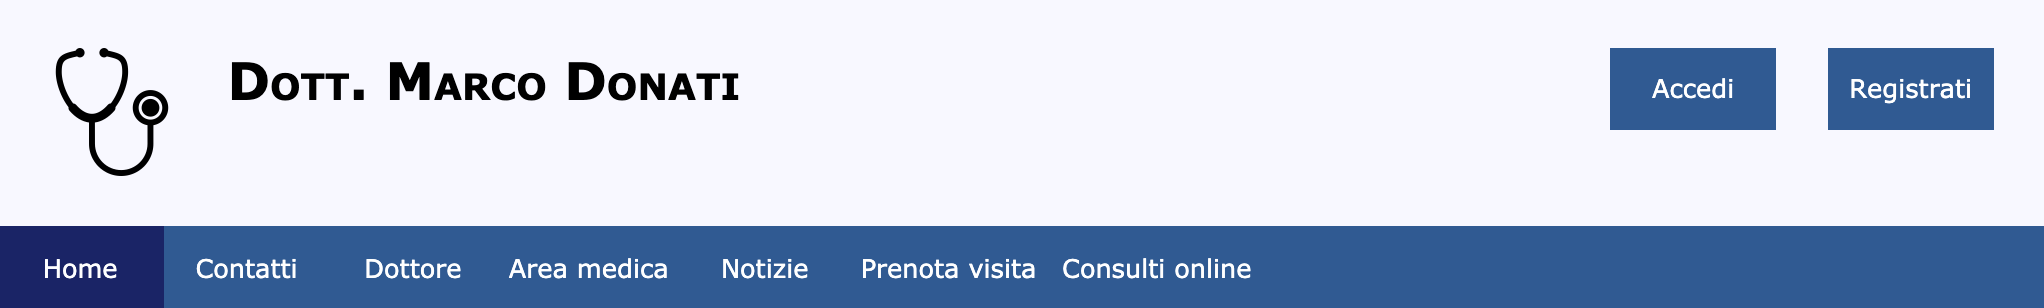
\includegraphics[width=12cm]{../img/header}
\end{center}
\captionof{figure}{Header}


\subsubsection{Breadcrumbs}
Le \textit{breadcrumbs} sono presenti in tutte le pagine del sito, sia mobile che desktop, e comprendono un insieme di campi che identificano la posizione dell’utente all’interno del sito. L’ultimo campo è la pagina corrente, ovvero la pagina che l’utente sta visualizzando. Per evitare link circolari, quest’ultimo campo è solo testuale.

\begin{center}

\includegraphics[width=12cm]{../img/bread1}
\end{center}
\captionof{figure}{Breadcrumbs utente non registrato}

\begin{center}

\includegraphics[width=12cm]{../img/bread2}
\end{center}
\captionof{figure}{Breadcrumbs utente registrato}

\subsubsection{Contenuto}
Lo schema che abbiamo utilizzato è quello a tre panelli, i quali corrispondono alle seguenti domande:
\begin{enumerate}
\item \textbf{Dove mi trovo?} la prima risposta a questa domanda si trova nel titolo della pagina .La seconda si trova nelle \textit{breadcrumbs}, che indicano il percorso fatto per arrivare in quel punto;
\item \textbf{Di cosa parla questa pagina?} la risposta a questa domanda si trova nello stesso contenuto della pagina, diviso solitamente in due colonne, una posizionata a sinistra per seguire le regole date dalla termografia e una a destra contenente un immagine. Questa disposizione è dettata anche dal fatto che il contenuto delle pagine web si comporta in modo opposto a quello fisico. Ad esempio nei giornali le immagini prendono gran parte della pagina poiché attirano maggiormente l'attenzione, mentre nel web è il testo a fare da leader nell’attenzione ricevuta. Questo viene definito effetto zapping. Il nostro sito cerca di evitarlo;
\item \textbf{Dove posso andare?} la risposta a questa domanda si trova nella \textit{navbar} ,la quale non cambia mai di posizione. \\
\end{enumerate}

\begin{center}
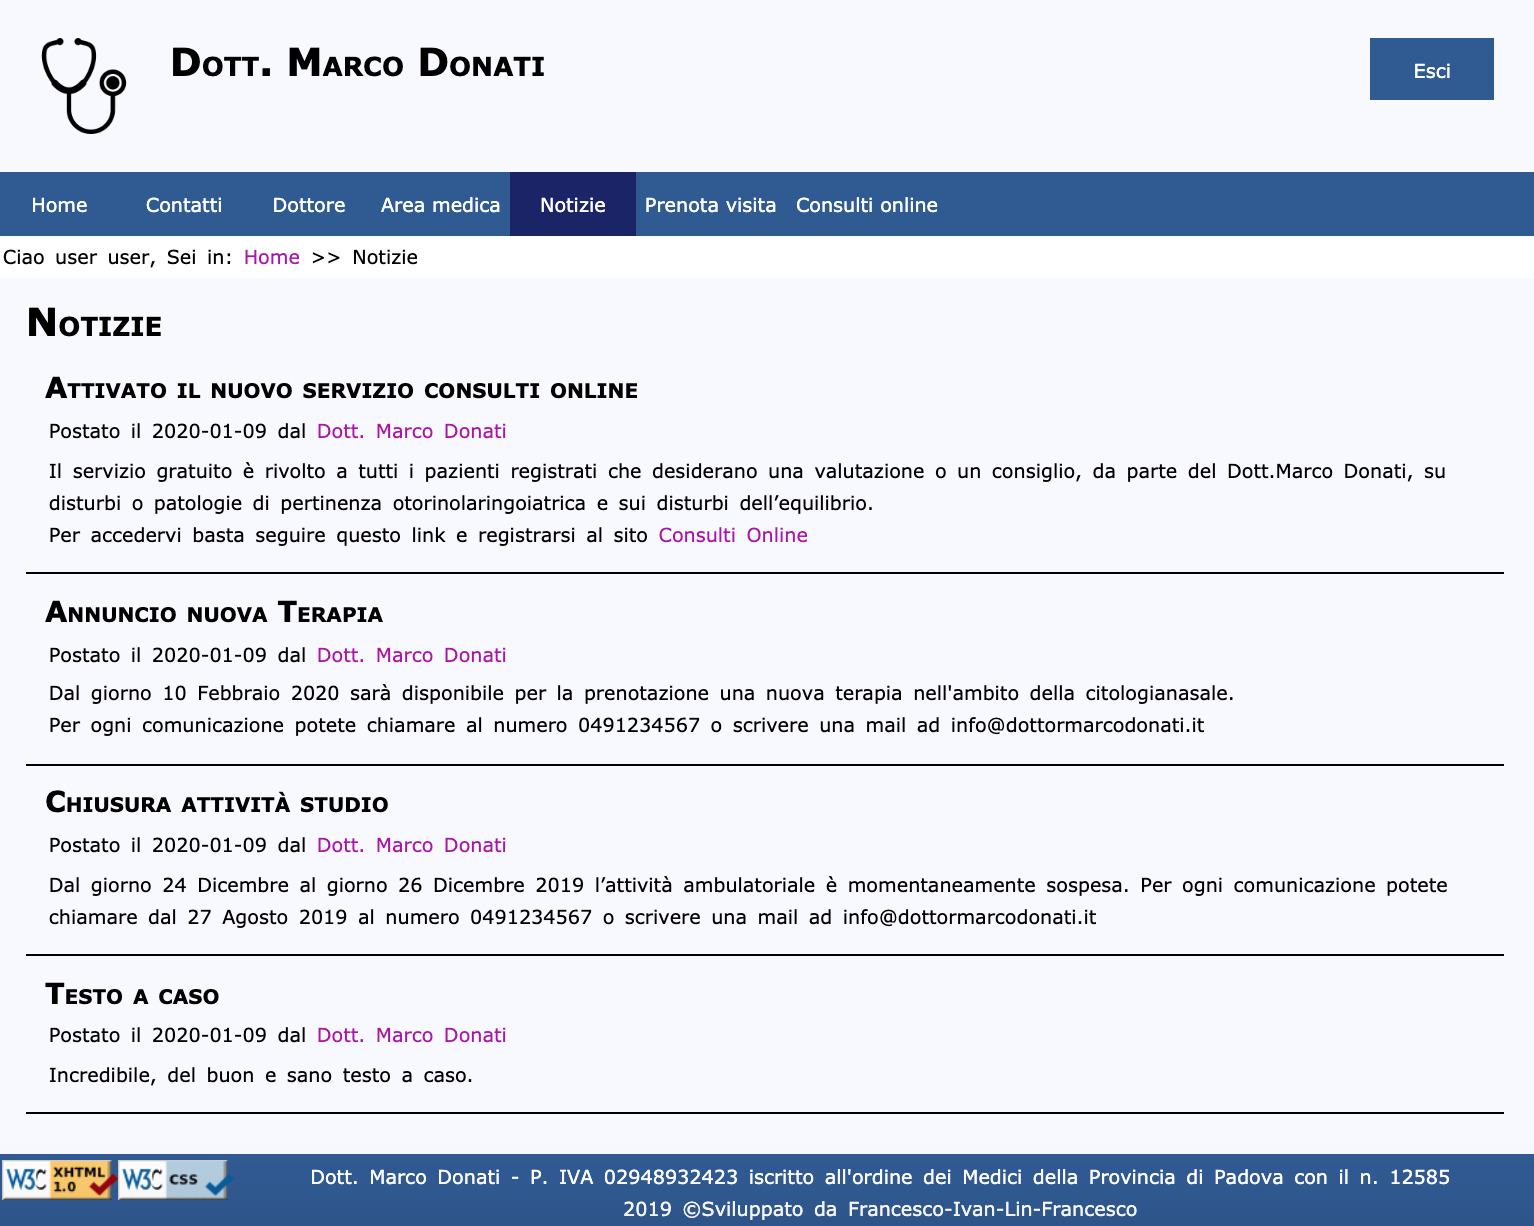
\includegraphics[width=12cm]{../img/contenuto}
\end{center}
\captionof{figure}{Esempio del contenuto di una pagina, in questo caso \textit{Notizie}} 

\bigskip

\textbf{Home} \\ 
Questa pagina ha la funzione di accogliere l’utente. È composta da uno \textit{slider} che mostra varie immagini del sito e da un testo che descrive il contenuto del sito sinteticamente.
Il testo è composto da meno di 100 parole, questo segue le regole base studiate da alcuni membri del gruppo durante il corso di WIM. Abbiamo quindi posto grande attenzione a restare nei limiti di tempo adeguati per mantenere l’attenzione degli utenti.
Infatti dopo vari studi è stato dimostrato che il tempo di permanenza in una pagina per il primo accesso da parte di un utente è 31 secondi; la nostra home in media rientra in questa tempistica. \\

\textbf{Pagina Contatti} \\ 
La funzione di questa pagina è di dare all’utente tutte le informazioni critiche su come contattare il dottore o trovare il suo studio medico.
Per fare ciò, oltre al testo contenente le varie informazioni, è stata inserita una mappa GoogleMaps interattiva. \\

\textbf{Pagina Dottore} \\
Questa pagina serve ad introdurre la figura del Dott. Marco Donati, illustrandone le competenze e achievement professionali. \\

\textbf{Pagina Area Medica} \\
La pagina Area Medica racchiude tutte le 4 prestazioni mediche fornite dal dottore. Si compone quindi di 4 link alle pagine singole (nelle quali le prestazioni vengono spiegate nel dettaglio) e di brevi descrizioni per ciascuna di esse. \\

\textbf{Pagina Notizie} \\
La pagina Notizie raccoglie tutte le news postate dal dottore. È fondamentale per gli utenti poiché comprende informazioni piuttosto importanti circa le chiusure straordinarie dello studio medico, oltre a fornire documentazione su nuove terapie e funzionalità del sito in sviluppo. \\

\textbf{Pagina Prenota Visita} \\
Questa pagina viene divisa in 2 colonne. Entrambe ospitano dei form;
questi guidano l’utente registrato (gli utenti non registrati non possono accedere alla pagina) nella scelta di una data per una visita specialistica.
Si deve scegliere anno, mese, giorno, prestazione specialistica e quindi l’orario. \\

\textbf{Pagina Consulti Online} \\
Questa pagina è dedicata interamente alla chat privata con il Dottore.
Può essere acceduta solo da utenti registrati.
Per ogni messaggio inviato viene mostrato nome utente, data e orario di invio. \\

\textbf{Pagina Accedi} \\
Questa pagina viene utilizzata per accedere al sito del dottore previa registrazione. Per accedere bisogna inserire email e password. \\

\textbf{Pagina Registrati} \\
Questa pagina viene utilizzata per registrarsi al sito del dottore.  Per registrarsi è necessario fornire nome, cognome, numero di telefono, email e password. \\


\subsubsection{Footer}
All’interno del footer compaiono le immagini di validazione W3C HTML, W3C CSS, le informazioni relative al dottore (partita IVA, numero di iscrizione all’ordine dei medici) e i nomi degli sviluppatori. Le immagini per la validazione sono link cliccabili, che una volta premuti validano la pagina rispettivamente in xHTML 1.0 e CSS 3.

\begin{center}

\includegraphics[width=12cm]{../img/footer}
\end{center}
\captionof{figure}{Footer}


\subsubsection{Database}
Il nostro database è composto dalle tabelle:
\begin{enumerate}
\item \textbf{Messaggi:} contiene tutti i messaggi dei Consulti Online (sia degli utenti, sia del dottore);
\item \textbf{Notizie:} contiene tutte le notizie postate dal dottore;
\item \textbf{Utenti:} contiene tutti le informazioni legate agli utenti registrati;
\item \textbf{Visite:} contiene tutte le visite prenotate da utenti registrati.
\end{enumerate}
